%% This is an example first chapter.  You should put chapter/appendix that you
%% write into a separate file, and add a line \include{yourfilename} to
%% main.tex, where `yourfilename.tex' is the name of the chapter/appendix file.
%% You can process specific files by typing their names in at the 
%% \files=
%% prompt when you run the file main.tex through LaTeX.
\chapter{Implementation}


		\subsection{Holding to the constraints}

	\section{Particle List Transpose}
As previously mentioned the particle list structure on the GPU is different than the structure on the CPU. On the GPU particles are stored in a structure of arrays, while on the CPU they are stored in a 6x$n$ array. This means that in order to copy a particle list generated on the CPU to the GPU, or vice versa, the particle list must be transposed. The two main places in the code where this matters is when the particle list is initially populated at the start of the code, and when copying a list of pre-calculated reinjection particles from the CPU to the GPU at every time step during the advancing phase.

The particle list transpose was implemented on the CPU in two different ways depending on the compiler used and the available libraries. A GPU based particle list transpose is significantly faster than a CPU based transpose. However, the GPU has a very limited amount of DRAM compared to the CPU, and it is preferable to use as much of the available GPU memory as possible for the main particle list. In any case transposing the entire particle list only occurs once, but a smaller transpose is performed every time step for reinjected particles. This means that while a faster transpose is preferable, it represents so little of the total computation time that it is not worth developing a complicated in place GPU transpose.  

	\section{Charge Assign}
	\label{sec:charge_assign}
	As previously mentioned, the charge assign is one of the most difficult funcitons to parallize. The niave approach of applying a thread to every particle and atomically adding each particles contribution to an array in global memory is very slow. Grouping the particles spatially allows the majority of the atomic operations to be done in the context of shared memory which is much faster than global memory. The resulting algorithm resembles basic domain decompositon where each thread-block represents a seperate sub-domain. The actual charge deposition method in this shceme is very similar to the niave approach, with a key difference being that all the threads in the thread block are operating on shared memory. Once all particles in the subdomain have contributed to grid in shared memory it takes only a small number of global memory accesses to write the contributions of a large number of particles to the main array $\chi$. 

	\subsection{Domain Decomposition}
		The primary grid is decomposed into sub-domains of size $nb_r, nb_{\theta}, nb_{\psi}$. The methods for determining the size of the sub-domains is outlined in section \ref{sec:grid_constraints}. The indexing of the sub-domains is done using a z-order curve in order to preserve spatial locality of the sub-domains in memory. This is done in an attempt to reduce the mean distance that particles must be moved in memory during the sort phase. A graphical representation of this is shown in figure \ref{fig:domain_decomp}.

\begin{figure}
\begin{center}
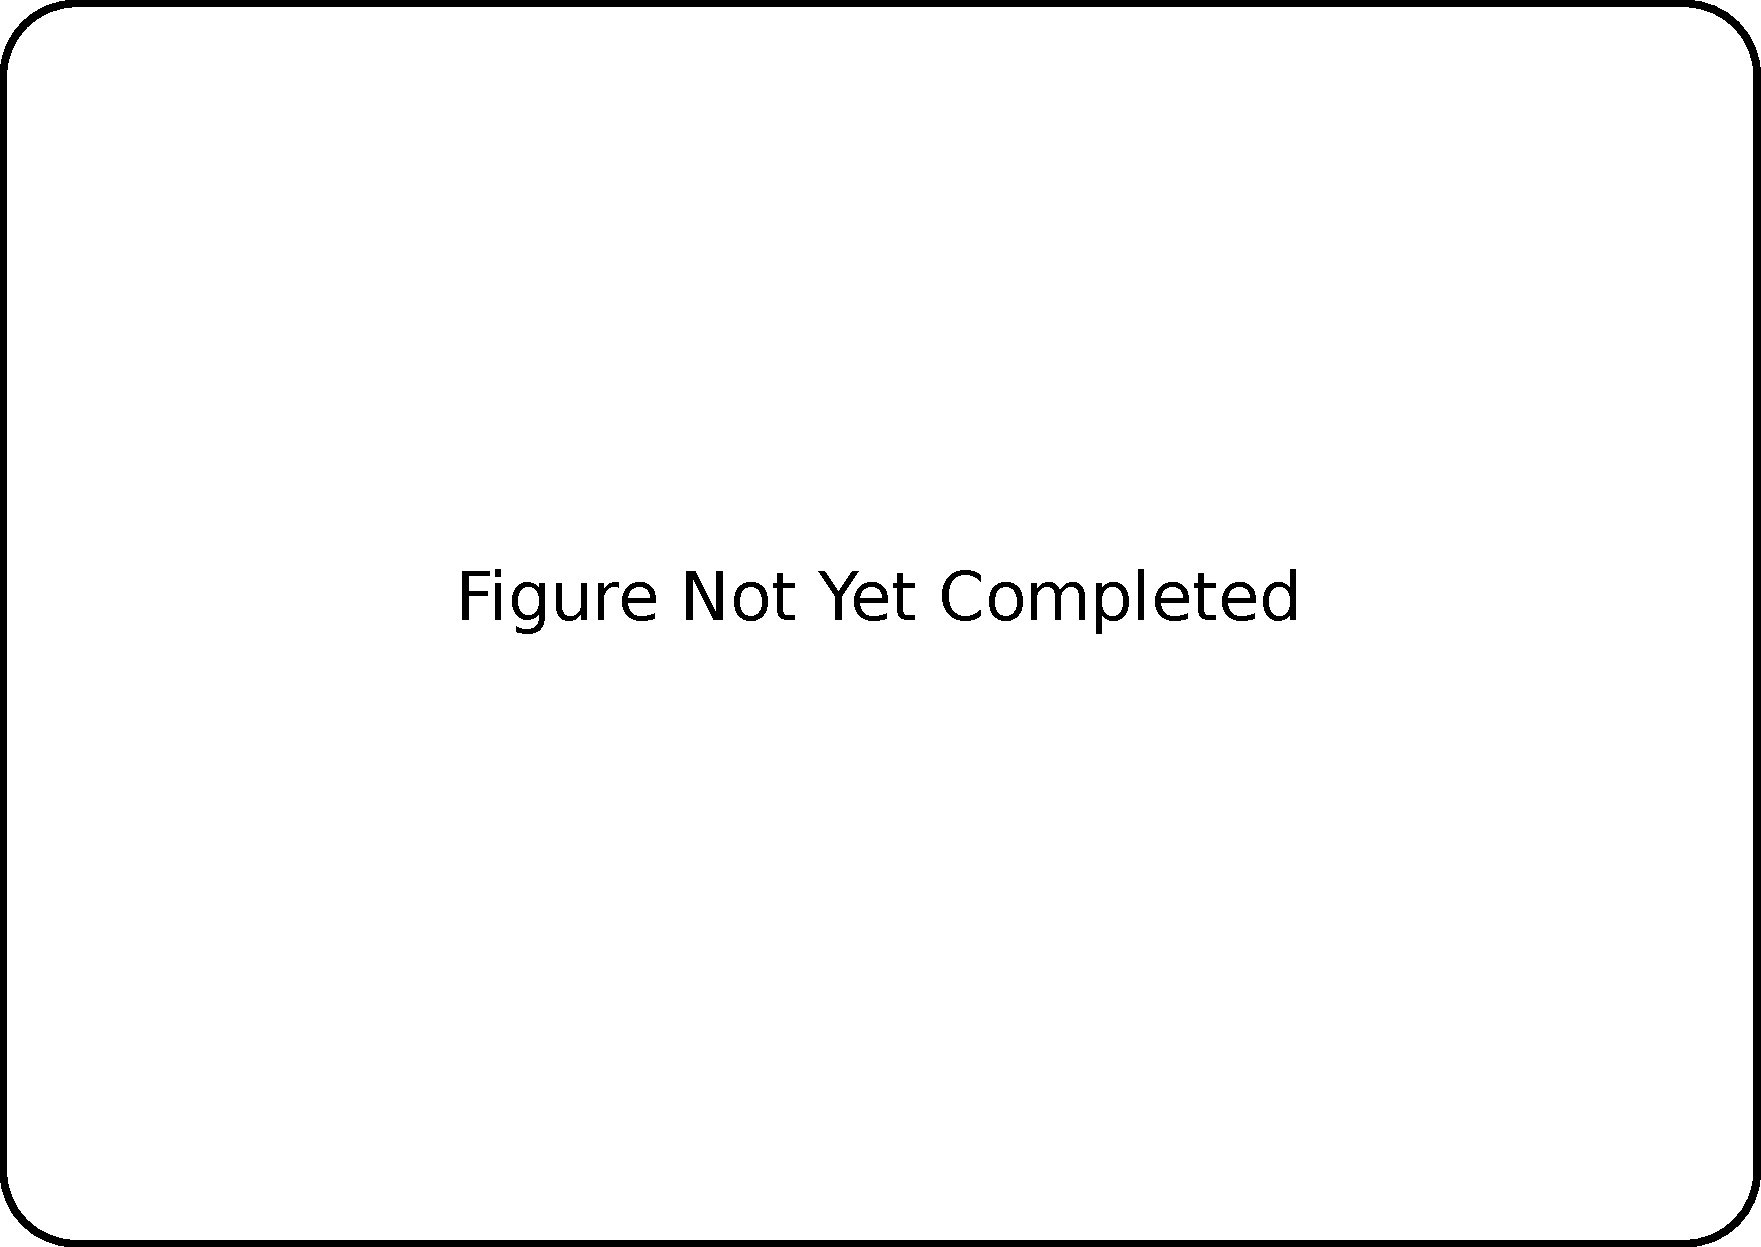
\includegraphics[width=4in]{introduction/not_finished.pdf}
\end{center}
\caption{Graphical Representation of domain decomposition and ParticleBin organization. Need to make figure}
\label{fig:domain_decomp}
\end{figure}

In addition to representing a sub-section of the computational mesh, each sub-domain must have a section of the particle list associated with it. The sub-domain must know all of the particles that reside within the region defined by that sub-domain. In essence each sub-domain represents a bin of particles that corresponds to some spatial location, hence the use of ``ParticleBin"  as the naming convention for these object.



	\subsection{Particle Bins}
The \emph{ParticleBin} object keeps track of all of the particles that reside in the region of space that the \emph{ParticleBin} represents. For the sake of simplicity all of the particle bins are the same size spatially, which means that the \emph{ParticleBin} object only has to keep track the section of the main particle list that the bin represents and the spatial origin of the bin. 

In the context of the particle list each bin represents a pair of bookmarks that bound a section of the particle list. The bookmarks for each bin are calculated after the particle list is sorted by algorithm \ref{alg:count_bins}.

\begin{algorithm}
	\caption{ParticleBin Bookmark Calculation}
	\label{alg:count_bins}
	\begin{algorithmic}
		\FORALL{  $\mathrm{threadID} = 0 \to \mathrm{ParticleList.nptcls}$ in \underline{parallel}}
			\STATE 
			\STATE $\mathrm{binID} = \mathrm{ParticleList.binID}[\mathrm{threadID}]$
			\STATE $\mathrm{binID_{left}} = \mathrm{ParticleList.binID}[\mathrm{threadID} - 1]$
			\STATE $\mathrm{binID_{right}} = \mathrm{ParticleList.binID}[\mathrm{threadID} + 1]$
			
			\IF{$\mathrm{binID} \neq \mathrm{binID_{left}}$}
				\STATE $\mathrm{ParticleBins[binID].ifirstp} = \mathrm{threadID}$
				\STATE $\mathrm{ParticleBins[binID_{left}].ilastp} = \mathrm{threadID} - 1$
			\ENDIF

			\IF{$\mathrm{binID} \neq \mathrm{binID_{right}}$}
				\STATE $\mathrm{ParticleBins[binID].ilastp} = \mathrm{threadID}$
				\STATE $\mathrm{ParticleBins[binID_{right}].ifirstp} = \mathrm{threadID} + 1$	
			\ENDIF
			
		\ENDFOR
	\end{algorithmic}
\end{algorithm}


The spatial origin of the bin is hashed using a z-order curve and stored as a 16-bit unsigned-integer. This 16-bit integer is refered to as the binID and is used for determining the region of the domain that a bin is responsible for as well as a sorting key for the particle list. Calculating the binID will be discussed in more detail in section \ref{sec:plist_sort}. A 16-bit unsigned integer is used for several reasons. First the sorting method detailed in section \ref{sec:plist_sort} is dependent on the number of bits of the sorting key. Second, the upper bound on the grid size set by using a 16-bit integer to store the z-order hash is much larger than the largest grid size that would need to be run. For a 16-bit integer this upper bound is $512^3$ grid points. The third reason for using a 16-bit integer is that it also reduces the memory requirements of the particle list by about 5\%, which does help when trying to run as many particles on the GPU as possible. 

	\subsection{Particle Push}
Now that the particles are organized spatially in memory, it is trivial to assign a single thread block to a region of space and corresponding particle bin in order to perform the particle push. This process is rather simple and is outlined in psuedo code in algorithm \ref{alg:gpu_c2mesh}. 

\begin{algorithm}
	\caption{GPU Charge Assign}
	\label{alg:gpu_c2mesh}
	\begin{algorithmic}
		\FORALL{ $ParticleBin \in Grid$ in \underline{parallel}}
			\STATE \emph{$\backslash \backslash$ Inside the threadBlock with ID blockID}

			\STATE \_\_shared\_\_ float $subGrid(nb_r,nb_{\theta},nb_{\psi})$

			\FORALL{ $node \in subGrid$ in \underline{parallel}}
			\STATE $node = 0$
			\ENDFOR
			
			\STATE \_\_syncthreads()
			

			\FORALL{  $particle \in ParticleBin$ in \underline{parallel}}
				\STATE cell = $particle.cell - ParticleBin.origin$
				\FORALL{ $node \in cell$}
					\STATE atomicAdd($subGrid(cell,node)$, weight($node$))
				\ENDFOR
			\ENDFOR
			\STATE \_\_syncthreads()

			\STATE \emph{$\backslash \backslash$ Write block results to global memory}
			\FORALL{ $node \in subGrid$ in \underline{parallel}}
				\STATE atomicAdd($Grid(blockID,node)$, $subGrid(node)$)
			\ENDFOR
			
		\ENDFOR
	\end{algorithmic}
\end{algorithm}

Each thread block reads in 512 particles at a time, although only 32 particles, a warp, are processed in parallel within the block. Each thread within this warp loops over the 8 nodes that bound the cell that contains the particle being processed. The nodes reside in a shared memory array, and are updated with the weighted particle data atomically. Once all of the nodes for a given particle have been updated the thread will retrieve a new particle from global memory. This process is repeated by all of the threads in the block until every particle in the particle bin has been processed. Once all of the particles have been processed the block then atomically updates the nodes in global memory with the values stored in shared memory.  

The atomic operations in this algorithm lead to some very interesting time complexity behavior. In essence this algorithm is being executed on a machine with 32 processors. The time complexity of this scenario is $\mathcal{O}(\frac{c}{p})$, where $c$ is constant and $p$ is the number of available processors. When two processors attempt to atomically update the same memory address, one of the processors must wait until the other is finished. This means that one processor is effectively lost for a 1-way conflict. 

The mean number of n-way atomic conflicts $N$ in a warp over a sub domain of size $G$, and the execution time $T$ is given by:
\begin{equation}
N = \frac{31!}{(31-n)! G^n} \hspace{0.1\textwidth} T(n) \propto \frac{c}{32-n}
\end{equation}

This means that the total time complexity of this algorithm with respect to the sub domain size $G$ is:

\begin{equation}
T(G) \propto c \cdot \sum_{n=1}^{31} \frac{1}{32-n} \frac{31!}{(31-n)! G^n}
\end{equation}

This behavior can be seen clearly in \ref{fig:subdomain_size_scan}. This algorithm on the GPU can perform the particle push up to 200x faster than the CPU version of the charge assign. However, this algorithm relies on the particle data being ordered spatially, which contributes to the run time. The method used to maintain an ordered particle list on the gpu will be discussed in the following section.


	\section{Particle List Sort}
	\label{sec:plist_sort}
	
	As previously mentioned in section \ref{sec:charge_assign} an ordered particle list must be maintained in order for the charge assign to be fast. The particle list sort, algorithm \ref{alg:sort_overview} consists of three distinct subroutines, populating the key/value pairs, sorting the key/value pairs, and finally a payload move. 

\begin{algorithm}
	\caption{Particle List Sort Overview}
	\label{alg:sort_overview}
	\begin{algorithmic}
		\STATE
		\STATE Populate\_KeyValues(Particles, Mesh, sort\_keys, sort\_values)
		\STATE
		\STATE thrust::sort\_by\_key(sort\_keys,sort\_keys+nptcls,sort\_values)
		\STATE
		\STATE Payload\_Move(Particles, sort\_values)
	\end{algorithmic}
\end{algorithm}

This method of maintaining particle list order was chosen because it is a good balance between simplicity and performance. An additional benefit of this routine is that it uses the sort from the thrust library, which is maintained by NVIDIA. 

		\subsection{Populating Key/Value Pairs}
The first step in sorting the particle list is ensuring that the key/value pairs needed by the sorting routine are populated. The sorting key for a particle is the index of the particle bin that the particle belongs to. Sorting values are simply the position of the particle in the unsorted list. 

Calculating the particle bin index, or binid, begins with calculating the mesh cell that the particle resides in. This cell described by coordinates $i_r, i_{\theta}, i_{\phi}$. The coordinates of the particle bin that a given cell resides in is given by:

\begin{equation}
ib_r = \frac{i_r}{nb_r} \mathrm{;}\hspace{0.5in} ib_{\theta} = \frac{i_{\theta}}{nb_{\theta}} \mathrm{;} \hspace{0.5in} ib_{\phi} = \frac{i_{\phi}}{nb_{\phi}}
\end{equation}

	The resulting block coordinates are then hashed using a z-order curve described in appendix A to give the binid. Each thread calculates the binid's for several particles and stores them in the sort\_keys array. Once a thread has calculated the binid for a particle it also stores the index of that particle as an integer in the sort\_values array. 

		\subsection{Sorting Key/Value Pairs}
		The key/value pair sorting is done using the thrust library sort\_by\_key template function. This function is provided by NVIDIA with CUDA. The thrust sort is a radix sort that has been optimized for NVIDIA GPUs\cite{NVIDIACorporation2011a}. The snippet of the sort code used in sceptic3Dgpu is shown in figure \ref{fig:thrust_sort}.

\begin{figure}
\begin{lstlisting}[frame=single]
	// wrap raw device pointers with a device_ptr
	thrust::device_ptr<ushort> thrust_keys(binid);
	thrust::device_ptr<int> thrust_values(particle_id);

	// Sort the data
	thrust::sort_by_key(thrust_keys,thrust_keys+nptcls,thrust_values);
	cudaDeviceSynchronize();
\end{lstlisting}
\vspace{-0.4in}
\caption{Thrust Sort Setup and Call}
\label{fig:thrust_sort}
\end{figure}


		\subsection{Payload Move}
		The payload move is responsible for moving all of the particles from their old locations in memory to the new sorted locations. The idea is simple, each thread represents a slot on the sorted particle list. Threads read in an integer, the particleID, from the values array that was sorted using the binid's. This integer is the location of a given threads particle data in the unsorted list. Data at index particleID is read in, and stored in the new list at index threadID. While the idea is simple, this algorithm would require a completely separate copy of the particle list, a lot of wasted memory. However, since the particle list is set up as a structure of arrays, there is something that can be done to significantly reduce the memory requirements. The method, outlined in algorithm \ref{alg:payload_move} reorders only a single element of the particle list structure at a time. 

\begin{algorithm}
	\caption{GPU Payload Move}
	\label{alg:payload_move}
	\begin{algorithmic}
		\FORALL{ $member \in XPlist$}
		\STATE float* idata = member
		\STATE float* odata = XPlist.buffer
		\STATE \textbf{reorder\_data}(odata,idata,particleIDs)
		\STATE member = odata
		\STATE buffer = idata
		\ENDFOR
	\end{algorithmic}
\end{algorithm}
  		
		Essentially the idea is that a great deal of time and memory can be saved by statically allocating a ``buffer'' array that is the same size as each of the data arrays. During the payload move each data array is sorted into the buffer array. Some pointer magic is performed, the old buffer array becomes the new data array, and the old data array becomes the buffer for the next data array. For sceptic3Dgpu this implementation of the payload move only increases the particle list size by about 8.6\%.



	\section{Poisson Solve}

	\section{Particle List Advance}
	
Moving the particles on the grid is fairly straightforward. The process starts with determining the acceleration of the particle. This is calculated by interpolating the potential, $\phi$, from the spherical mesh using the same methods as the cpu code. The new position of the particle is simply $\vec{x}' = \vec{x}+\vec{v}\Delta t+\frac{1}{2}\vec{a}\Delta t^2$. A more detailed description of the basics of the particle advance can be found in reference \ref{Patacchini2007} section 3.1.2.
		
While the implementation of the basic physics of the particle advance remains the same, there were several interesting issues. Quickly determining whether a particle has crossed one of the domain boundaries, contributing to diagnostic outputs, and handling reinjections were the main issues. 

		\subsection{Checking Domain Boundaries}
In order to correctly contribute to the diagnostic outputs, the location where a particle left the domain must be known. This means that the process or checking whether or not a particle has left the grid must also calculate the position of the particle when it crossed the boundary. This is handled differently for the inner and outer boundaries. 

The outer boundary is fairly straightforward. A particle has left the domain if the radial position of the particle $r$ is greater than the maximum radius of the domain $r_{max}$. The 

		\subsection{Diagnostic Outputs}
		\subsection{Handling Reinjections}
Once it has been determined that particles have left the grid, new particles must be reinjected to replace them. In the serial version of the code this is handled by simply calling a reinjection subroutine that determines the new particle's position and velocity. Once the new position and velocity has been found the particle is moved for the remainder of the time step, and be replaced by a new particle if the reinjected particle leaves the domain.  

Performing reinjections in this manner on the GPU would introduce very large divergences in warp execution as well as very uncoalesced memory accesses. Eliminating the warp divergences requires that all of the threads in a warp be operating on reinjected particles. Reducing the uncoalesced memory accesses would require that all of the reinjected particles be adjacent in memory. Since we already have an object with methods that can move a list of particles and handle reinjections, all we really need is some method by which we can efficiently and reversibly ``pop" a subset of the particles in the main list to a secondary list. From there we can perform the particle advance on the secondary list, and place the results back in the empty particle slots in the main list. The resulting advancing algorithm is as follows:

\begin{algorithm}
	\caption{Particle Advancing Algorithm}
	\label{alg:advancing}
	\begin{algorithmic}
		\STATE // Update The particle positions and check domain boundaries
		\STATE $\textbf{GPU\_Advance}(particles,mesh,Exit\_Flags)$
		\STATE
		\STATE \textbf{Prefix\_Scan}(Exit\_Flags)
		\STATE
		\STATE nptcls\_reinject = Exit\_Flags[nptcls-1]
		\STATE
		\IF{nptcls\_reinject $>$ 0}
			\STATE
			\STATE reinjected\_particles.allocate(nptcls\_reinject)
			\STATE
			\STATE \textbf{Stream\_Compact}(particles $\subset$ exited $\rightarrow$ reinjected\_particles)
			\STATE
			\STATE // Recursivley call the Advance on the reinjected particles
			\STATE reinjected\_particles.advance()
			\STATE
			\STATE \textbf{Stream\_Expand}(reinjected\_particles $\rightarrow$ exited $\supset$ particles)
		\ENDIF
		\STATE
		\STATE return
	\end{algorithmic}
\end{algorithm}

Compacting some subset of a parent list is a fairly easy parallel operation called stream compaction. 

\begin{figure}
\begin{center}
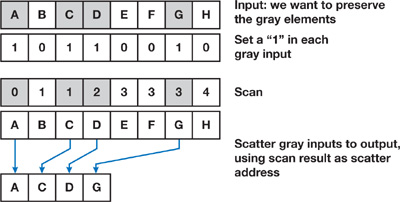
\includegraphics[width=4in]{implementation/stream_compact.jpg}
\end{center}
\caption{Stream Compaction from GPU Gems 3 \cite{Harris2007}}
\label{fig:stream_compact}
\end{figure}

Stream compaction, shown in figure \ref{fig:stream_compact} is a process by which a random subset of a list can be quickly copied to a new list in parallel. It only works for some binary condition, such as an array of length nptcls, where each element is 1 for particles that have left the domain, and 0 for all others. For each `true' element taking the cumulative sum of all preceding elements yields a unique number that can be used as an index in a new array. 

The new positions and velocities for reinjected particles are taken from a precalculate pool of new particles. This pool is approximately 1/10\textsuperscript{th} the size of the main particle list, and is repopulated prior to every advance step. Prior to the first advance step the entire pool is populated, but subsequent steps only refill slots that have been used in reinjections. This ``pool" method was chosen over implementing the reinjection calculations on the GPU for reasons of code maintenance. There are currently several different reinjection schemes that sceptic3D can call. Maintaining versions of those routines in both fortran and CUDA would be more cumbersome than the small benefit that calculating them on the GPU would provide. 




